\scanpage{81}
\mspage{329}

$3^\circ)$ We then construct
\[
h_0=\xi^{-1}\ell_0^{\gamma}
\in\widehat{\Pi}_{0,3}
\]
The relation in $2^\circ)$ ensures that $h_0\sigma_\infty(h_0)=1$ i.e.
that $h_0$ can be put in the form
\[
h_0=\sigma_\infty(g_0)^{-1}g_0
\]
\unsure{with} $g_0\in\widehat{\Pi}_{0,3}$.

\margin{N.B. We should make sure on the other hand that knowledge of $g_0$
does \unsure{not} determine $\gamma$ i.e. $p$
i.e. that \deleted{\illegible{2}} the $\gamma$
such that $\xi=\ell_0^{\gamma}h_0^{-1}$
\unsure{satisfies} (A) is \unsure{not} \deleted{\illegible{1}} unique.
To be clarified!}

$4^\circ)$ We can now put
\[
g=\sigma_\infty(g_0)\ell_1^{\gamma}\rho(g_0)^{-1}
=(g_0\ell_0^{-\gamma})\xi
\rho(g_0\ell_0^{-\gamma})^{-1}
\]
and we \deleted{\unsure{define}} have what is needed to define $u$, via
\[
\left\{
\begin{aligned}
u(\sigma_\infty)&=\sigma_\infty\\
u(\rho)&=g\rho
\end{aligned}
\right.
\]

Here, the only delicate equation, \deleted{for} which
the existence (not the uniqueness, in the good case) of a solution, is problematic,
is equation C (in $\gamma\in\widehat{\mathbb Z}$)
--- plus the further condition that $2\gamma+1\in\widehat{\mathbb Z}^{*}$.
This is therefore a \deleted{\unsure{question}}\inserted{\uline{condition}}
on $\lambda\in\widehat{\Pi}_{0,3}$ --- or rather two types of condition,
according as $\xi$ is defined in terms of $\lambda$ by
one or the other formula (B).

I expect that we are in one or

\margin{80}

\scanpage{82}

the other case of formulas (B), according as $p\bmod 3$ is congruent to $1$, or to $-1$
(N.B. it must not be congruent to $0$, since $p\bmod 3\in(\mathbb Z/3\mathbb Z)^*$)
i.e. according as $2\gamma\equiv 0$ or $-2$ $(3)$ i.e.
$\gamma\equiv 0$ or $-1$ $(3)$
(N.B. $\gamma$ must not be $\equiv 1$ $(3)$,
otherwise $2\gamma+1=p$ would be congruent to $0\bmod(3)$).
This is in any case what \unsure{will be} the case if $u\in\Gamma_{\mathbb Q_0}$.

To test this, let us reduce the \deleted{\illegible{1}}\inserted{group}
$\widehat{\mathfrak S}_{0,3}^{+}$
modulo the\deleted{es}\inserted{'} \unsure{equation|equations}
$\ell_0^3=1$ i.e. $(\sigma_\infty\rho)^6=1$
\[
\deleted{\ell_0^3=\ell_1^3=\ell_\infty^3=1\quad\ell_\infty}
\]
so that $\widehat{\mathfrak S}_{0,3}^{+}$
is \unsure{replaced} by an extension of $\mathfrak S_3$
by the group defined by the generators $\ell_0,\ell_1,\ell_\infty$ satisfying
\[
\unsure{\ell_0}^3=\ell_1^3=\ell_\infty^3=(\ell_\infty\ell_1\ell_0)=1
\]
--- or better, let us use
\[
\widehat{\mathfrak S}_{0,3}^{+}
\simeq\mathrm{Sl}(2,\mathbb Z)^{\prime\,\wedge}
\]
and reduce directly in
\[
\mathrm{Sl}(2,\mathbb Z/6\mathbb Z)'
\simeq\mathrm{Sl}(2,\mathbb Z/2\mathbb Z)
\times\mathrm{Sl}(2,\mathbb Z/3\mathbb Z)'.
\]

\margin{81}

\scanpage{83}
\mspage{330}

But to do the calculations, we must be able to identify $\sigma_\infty$
\inserted{and} $\rho$ as elements of
$\mathrm{Sl}(2,\unsure{\widehat{\mathbb Z}|\mathbb Z})$
--- an explicitation which we shall carry out presently.

\begin{center}\rule{2cm}{0.4pt}\end{center}

Returning to (24 bis), and putting
$\unsure{h_0|h_\infty}=\xi^{-1}\ell_0^{\gamma}$ into it, we get
\[
\tag{61}
g_0=\widehat{\varphi}(\xi)
\varepsilon_0^{\gamma-\beta}
\]
We thus think that $u$ corresponds to
$(\xi,g_0,\gamma,\beta)$,
with $\xi,g_0\in\widehat{\Pi}_{0,3}$
and $\gamma,\beta\in\widehat{\mathbb Z}$
\margin{\illegible{1}}
satisfying
\[
\tag{62}
\left\{
\begin{aligned}
&\xi\rho(\xi)\rho^2(\xi)=1\\
&\xi\underbrace{\sigma_\infty(g_0)^{-1}g_0}_{h}
=\ell_0^{\gamma}\\
&\deleted{\unsure{\widehat{\varphi}(\xi)}}g_0
=\widehat{\varphi}(\xi)
\varepsilon_0^{\gamma-\beta}\\
&2\gamma+1\in\widehat{\mathbb Z}^{*}
\end{aligned}
\right.
\]
from which we can eliminate $g_0$, and we find equations in
$(\xi,\deleted{\gamma}r,\deleted{\beta}s)$
$(r=\gamma-\beta,\ s=\gamma+\beta)$
\[
\tag{63}
\left\{
\begin{aligned}
&\xi\rho(\xi)\rho^2(\xi)=1\\
&\sigma_\infty\bigl(\widehat{\varphi}(\xi)\bigr)^{-1}
\widehat{\varphi}(\xi)
=\varepsilon_1^r\xi^{-1}\varepsilon_0^s\\
&\underbrace{r+s+1}_{p}\in\widehat{\mathbb Z}^{*}
\end{aligned}
\right.
\]
\margin{(thus $\xi=\lambda\rho(\lambda)^{-1}$
or $\xi=\lambda\ell_0^{-1}\rho(\lambda)^{-1}$}

Here, $\unsure{\lambda}$ is determined modulo transformation into
$\lambda'=\deleted{\unsure{\ell_0^{\alpha}\xi}}\ell_0^\alpha\lambda$
thus $\xi$ becomes
$\xi'=\ell_0^\alpha\xi\ell_1^{-\alpha}$

\margin{82}

\scanpage{84}
\mspage{331}

\uline{42} Recapitulation on the group
\[
(\mathfrak S_{0,3})
\simeq
\bigl(\Pi_1(U_{0,3}^{\mathrm{an}},\mathfrak S_3;-\bar j)\bigr)
\simeq
\bigl(\widetilde\Pi'_{0,3}\simeq
\Pi_1((\mathbb P^{1\mathrm{an}},0\{0\}+2\{1\}+3\{\infty\}),\unsure{\{1,\tau\}};-\bar j)\bigr)
\]
\[
\simeq\bigl(\mathrm{Gl}(2,\mathbb Z)'=\mathrm{Gl}(2,\mathbb Z)/\{\pm1\}
\simeq\mathrm{GP}(1,\mathbb Z)\bigr)
\simeq\bigl(\mathcal T'_{1,1}=\mathcal T_{1,1}/\{\pm1\}\bigr)
\]
and on the ``loop'' automorphisms of
$\widehat{\mathfrak S}_{0,3}^{+}$ and of
$\widehat\Pi_{0,3}$ (Fundamental formulary).

\margin{\deleted{\illegible{1}} $\mathfrak S_{0,3}$ defined as $\mathrm{Aut}_{\mathrm{lac}}(\Pi_{0,3})$ --- we give \uline{five} different \unsure{views} of it ! (In fact, there are \uline{some} ten of them, cf. (V) below\ldots)}

\uline{I}) $\mathcal T_{0,3}$

The group $\mathfrak S_{0,3}$ is \unsure{presented} as an extension
\[
(1)\qquad
\diagram{\begin{tikzcd}[ampersand replacement=\&,column sep=small]
1 \arrow[r,dash] \& \Pi_{0,3} \arrow[r] \arrow[d,phantom,"\Vert"] \& \mathfrak S_{0,3} \arrow[r] \& \mathcal T_{0,3} \arrow[r] \arrow[d,phantom,"\wr"] \& 1 \\
\& \Pi_1(U_{0,3}^{\mathrm{an}};-\bar j) \&\& \mathfrak S_3\times\mathbb Z/2\mathbb Z \&
\end{tikzcd}}
\]
where $\mathfrak S_3\times\mathbb Z/2\mathbb Z$ is regarded as a group operating on
$U_{0,3}^{\mathrm{an}}=\mathbb P^{1\mathrm{an}}\setminus\{0,1,\infty\}=\mathbb C\setminus\{0,1\}$,
\deleted{by holomorphic \unsure{automorphisms}}
\deleted{$\mathfrak S_3$ operating by permutations}
--- it is the group of conformal automorphisms \unsure{of the|of} $\mathbb P^{1\mathrm{an}}$ which stabilize $\{0,1,\infty\}$.
The group \margin{\unsure{(2)}}\deleted{\unsure{$\mathfrak S_3$}}\inserted{$\mathfrak S_3=\mathfrak S_{\{0,1,\infty\}}$} is the subgroup of \deleted{\unsure{elements}}conformal automorphisms, it is identified with the group of permutations of $\{0,1,\infty\}$, its six elements are
\unsure{$\mathrm{id}$;|$1$;}
$\dot\sigma_0,\dot\sigma_1,\dot\sigma_\infty$ (\inserted{the three} transpositions),
$\dot\rho,\deleted{\unsure{\dot{\rho}}}\dot\rho^{-1}$ (cyclic permutations)
given by the explicit formulas
\[
(2)\qquad
\left\{\begin{array}{l}
\dot\sigma_0(z)=\dfrac{z}{z-1}\inserted{\unsure{=1+\dfrac{1}{1-z}|=1+\dfrac{1}{z-1}}},\quad
\dot\sigma_1(z)=\dfrac1z,\quad
\dot\sigma_\infty(z)=1-z,\\[4pt]
\dot\rho(z)=\dfrac1{1-z},\quad
\dot\rho^{-1}(z)=1-\dfrac1z=\dfrac{z-1}{z},
\end{array}\right.
\]
with
\[
(3)\qquad
\left\{\begin{array}{l}
\dot\sigma_0\dot\sigma_1=\dot\sigma_1\dot\sigma_\infty=\dot\sigma_\infty\dot\sigma_0=\dot\rho,\\
\dot\rho\dot\sigma_0\dot\rho^{-1}=\dot\sigma_1,\quad
\dot\rho\dot\sigma_1\dot\rho^{-1}=\dot\sigma_\infty,\quad
\dot\rho\dot\sigma_\infty\dot\rho^{-1}=\dot\sigma_0
\end{array}\right.
\]
\[
(4)\qquad
\dot\sigma_0^2=\dot\sigma_1^2=\dot\sigma_\infty^2=\dot\rho^3=1.
\]
The group $\mathcal T'_{0,3}=\mathbb Z/2\mathbb Z\subset\mathcal T_{0,3}$ appears as the center,
\margin{83}

\scanpage{85}

it is generated by complex conjugation $\tau$
\[
(5)\qquad ,\quad \tau(z)=\bar z,
\]
the five other elements of $\mathcal T_{0,3}$ are
\[
\deleted{\unsure{\tau\sigma}}\quad(6)\qquad
\tau\dot\sigma_0=\dot\tau_0,\quad
\tau\dot\sigma_1=\dot\tau_1,\quad
\tau\dot\sigma_\infty=\dot\tau_\infty,\quad
\tau\rho,\quad\tau\rho^{-1}=(\tau\rho)^{-1},
\]
the \unsure{anti-involutions|anti-involutions} $\tau'_i$ $(i=0,1,\infty)$ are particularly interesting, \unsure{given} by
\[
(7)\qquad
\unsure{\dot\tau'_0(z)}=\frac{\bar z}{\bar z-1},\quad
\unsure{\dot\tau'_1(z)}=\frac1{\bar z},\quad
\dot\tau'_\infty(z)=1-\bar z.
\]

The fixed points \deleted{\unsure{in $U_{0,3}$}} of the \inserted{\illegible{1}} conformal automorphisms of \deleted{\illegible{2}} $(\mathbb P^{1\mathrm{an}},\{0,1,\infty\})$ are the following
\[
(8)\qquad
\left\{\begin{array}{l}
(\mathbb P^1_{\mathbb C})^{\dot\sigma_0}=\{0,2\},\quad
(\mathbb P^1_{\mathbb C})^{\dot\sigma_1}=\{1,-1\},\quad
(\mathbb P^1_{\mathbb C})^{\dot\sigma_\infty}=\{\infty,\frac12\}\\[3pt]
\mathbb P_{\mathbb C}^{1\,\dot\rho}=\mathbb P^{1\,\dot\rho^{-1}}=\{-\bar j,-j\}
\end{array}\right.
\qquad
\begin{array}{l}
\text{where }j=\exp 2i\pi/3=\dfrac{-1+i\sqrt3}{2}\quad\text{primitive root}\quad\text{$3^{\unsure{\mathrm{ième}|\mathrm{ème}}}$ of $1$}\\[5pt]
-\bar j=\exp 2i\pi/6=\dfrac{1+i\sqrt3}{2}\quad\text{primitive root}\quad\text{$6^{\unsure{\mathrm{ième}|\mathrm{ème}}}$ of $1$}
\end{array}
\]

\margin{N.B. $\mathbb P_{\mathbb C}^{1\,\dot\rho\tau}=\mathbb P_{\mathbb C}^{1\,\dot\rho^{-1}\tau}=\varnothing$}

\[
(9)\qquad
\left\{\begin{array}{l}
\mathbb P_{\mathbb C}^{1\,\tau}=\mathbb P_{\mathbb R}^{1}\\[3pt]
\mathbb P_{\mathbb C}^{1\,\dot\tau'_0}=\{x+iy\mid(x-1)^2+y^2=1\}
\inserted{=\{z\mid z+\bar z=z\bar z\}\unsure{=\frac1z|=\frac12}}
\inserted{\unsure{=\frac12-\mathbb U}},\quad
\mathbb P_{\mathbb C}^{1\,\dot\tau'_1}=\{z\mid z\bar z=1\}=\{x+iy\mid x^2+y^2=1\}=\mathbb U\\[3pt]
\mathbb P_{\mathbb C}^{1\,\dot\tau'_\infty}=\{z\mid z+\bar z=1\}=\{x+iy\mid x=\frac12\}=\frac12+i\mathbb R;
\end{array}\right.
\]

The most suggestive picture is probably that of the Riemann sphere, where $\tau,\dot\tau'_0,\dot\tau'_1,\dot\tau'_\infty$ appear as the \deleted{\unsure{symmetries}}\inserted{\uline{reflections}} with respect to the corresponding \deleted{``equators''}\inserted{``\unsure{gr\textsuperscript{eat}|great} circles''}, which for $\tau$ is ``the equator'' and for the others are the great circles \inserted{``meridians''}, passing through the poles $-\bar j,-j$, which effect the cutting up of the equator into six circular segments, by the subdivision points $0,\frac12,1,2,\infty,-1$.

\figure{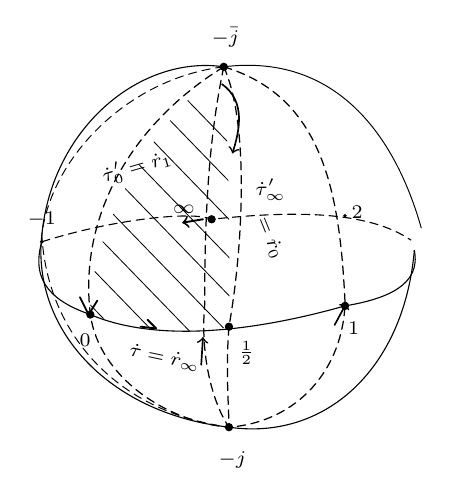
\begin{tikzpicture}[x=.022cm,y=-.022cm,line cap=round,line join=round,font=\scriptsize]
\coordinate (N) at (110,8);
\coordinate (S) at (113,216);
\draw[line width=.4pt] (N) .. controls (62,1) and (11,43) .. (5,105)
 .. controls (-1,158) and (42,208) .. (S)
 .. controls (168,224) and (214,183) .. (220,114);
\draw[line width=.35pt] (N) .. controls (175,0) and (209,48) .. (224,101);
\begin{scope}
\clip (N) .. controls (62,47) and (32,109) .. (33,151)
 .. controls (60,160) and (91,164) .. (113,158)
 .. controls (114,100) and (112,43) .. (N);
\foreach \a in {-80,-58,-36,-14,8,30,52,74,96,118,140,162}
  \draw[line width=.3pt] (-15,\a)--(145,{\a+165});
\end{scope}
\draw[dash pattern=on 3pt off 2pt,line width=.45pt] (N)
 .. controls (58,40) and (26,93) .. (33,151)
 .. controls (38,187) and (77,213) .. (S);
\draw[dash pattern=on 3pt off 2pt,line width=.45pt] (N)
 .. controls (101,51) and (99,95) .. (99,145)
 .. controls (96,180) and (106,206) .. (S);
\draw[dash pattern=on 3pt off 2pt,line width=.45pt] (N)
 .. controls (125,41) and (121,113) .. (113,158)
 .. controls (111,183) and (113,205) .. (S);
\draw[dash pattern=on 3pt off 2pt,line width=.45pt] (N)
 .. controls (167,25) and (177,80) .. (180,144)
 .. controls (179,182) and (153,213) .. (S);
\draw[dash pattern=on 3pt off 2pt,line width=.35pt] (N)
 .. controls (53,15) and (10,62) .. (5,105)
 .. controls (8,161) and (47,207) .. (S);
\draw[dash pattern=on 3pt off 2pt,line width=.4pt] (5,109)
 .. controls (46,96) and (92,91) .. (103,96)
 .. controls (150,91) and (193,91) .. (218,108);
\draw[line width=.4pt] (5,109) .. controls (-2,133) and (13,144) .. (33,151)
 .. controls (80,171) and (148,155) .. (180,146)
 .. controls (204,142) and (224,134) .. (220,114);
\draw[->,line width=.7pt] (98,96)--(86,98);
\draw[->,line width=.6pt] (109,18) .. controls (123,28) and (119,45) .. (115,58);
\draw[->,line width=.6pt] (97,180)--(98,164);
\draw[->,line width=.6pt] (174,157)--(181,144);
\draw[line width=.65pt] (27,141)--(32,151)--(37,143);
\draw[line width=.65pt] (62,158)--(71,159)--(66,154);
\foreach \p in {(110,8),(113,216),(103,96),(33,151),(113,158),(180,146)}
  \fill \p circle[radius=2.4];
\foreach \p in {(5,109),(180,94)}
  \fill \p circle[radius=1.1];
\node[inner sep=0pt] at (111,-9) {$-\bar j$};
\node[inner sep=0pt] at (115,235) {$-j$};
\node[inner sep=0pt] at (5,96) {$-1$};
\node[inner sep=0pt] at (87,90) {$\infty$};
\node[inner sep=0pt] at (187,92) {$2$};
\node[inner sep=0pt] at (30,166) {$0$};
\node[inner sep=0pt] at (123,173) {$\frac12$};
\node[inner sep=0pt] at (185,159) {$1$};
\node[inner sep=0pt,rotate=16] at (60,66) {$\dot\tau'_0=\dot r_1$};
\node[inner sep=0pt] at (137,79) {$\dot\tau'_\infty$};
\node[inner sep=0pt,rotate=-68] at (137,107) {$=\dot r_0$};
\node[inner sep=0pt,rotate=-12] at (76,176) {$\unsure{\dot\tau}=\unsure{\dot r}_\infty$};
\end{tikzpicture}}

Let us also note the formulas
\[
(10)\qquad
\left\{\begin{array}{l}
\dot\rho\dot\tau'_0\dot\rho^{-1}=\dot\tau'_1,\quad
\dot\rho\dot\tau'_1\dot\rho^{-1}=\dot\tau'_\infty,\quad
\dot\rho\dot\tau'_\infty\dot\rho^{-1}=\dot\tau'_0\\[3pt]
\dot\tau'_0\dot\tau'_1=\dot\tau'_1\dot\tau'_\infty=\dot\tau'_\infty\dot\tau'_0=\dot\rho
\end{array}\right.
\]
\margin{84}

\scanpage{86}
\mspage{332}

The four great circles (9) cut the sphere into 12 spherical triangles, which form fundamental domains for the group $\mathcal T_{0,3}\simeq\mathfrak S_3\times\mathbb Z/2$ of order 12, and are permuted among themselves in a simply transitive way.
\deleted{\unsure{Taking|Let us take} one of}\inserted{(This is \unsure{also|thus}} the barycentric subdivision of the double spherical triangles \unsure{determined} by the equator $\mathbb P_{\mathbb R}^{1}$, and its three subdivision points $0,1,\infty$.)
Let us take one of these spherical triangles, say $(-\bar j,0,\frac12)$, the reflections with respect to its \inserted{three} sides, i.e.
$\tau,\dot\tau'_\infty,\dot\tau'_0$, form a system of generators of $\mathcal T_{0,3}$, with the relations
\[
(11)\qquad
\tau^2=\dot\tau_\infty^{\prime 2}=\dot\tau_0^{\prime 2}
=\left(\underbrace{\unsure{\tau}\dot\tau'_\infty\tau}_{\dot\sigma_\infty}\right)^2
=\left(\underbrace{\dot\tau'_0\dot\tau'_\infty}_{\dot\rho^{-1}}\right)^3
=\left(\underbrace{\tau\unsure{\dot\tau'_0}\deleted{\unsure{\tau}}}_{\dot\sigma_0}\right)^2=1
\]

as for $\mathfrak S_3=\mathcal T_{0,3}^{+}$, it is generated by
$\tau\dot\tau'_\infty=\dot\sigma_\infty$, $\dot\tau'_0\dot\tau'_\infty=\dot\rho^{\unsure{-1|1}}$ and $\tau\dot\tau'_0=\dot\sigma_0$, with the relations
\[
(12)\qquad
\dot\sigma_0\dot\rho\dot\sigma_\infty=\dot\sigma^2=\dot\rho^3=\dot\sigma_0^2=1.
\]

\uline{II}) The group $\Pi_{0,3}$ is generated by $\ell_0,\ell_1,\ell_\infty$, linked by the generating relation
\[
(13)\qquad \ell_\infty \ell_1\ell_0=1
\]
The \deleted{group} subgroup \inserted{of index 2}
$\mathfrak S'_3=(\mathcal T_{0,3})_{-\bar j}=\unsure{\mathcal T_{0,3}}$,
stabilizer of $-\bar j$, consisting of the $(g,\tau^\varepsilon)\in\mathfrak S_3\times\mathbb Z/2\mathbb Z$ such that $\mathrm{sg}(g)=(-1)^\varepsilon$, operates on $\Pi_{0,3}$.
This subgroup consists of $1,\dot\tau_0,\dot\tau_1,\dot\tau_\infty,\dot\rho,\dot\rho^{-1}$, and their operations on $\Pi_{0,3}$ are denoted respectively $1,\tau'_0,\tau'_1,\tau'_\infty,\rho,\rho^{-1}$.

\margin{\uline{N.B.} $\tau'_0,\tau'_1,\tau'_\infty$ were previously denoted (in [C]) $\unsure{\sigma_0,\sigma_1,\sigma_\infty|\bar\sigma_0,\bar\sigma_1,\bar\sigma_\infty}$.}
\margin{85}

\scanpage{87}

\deleted{(14)}\quad\deleted{$\rho(\ell_0)=$}
We identify these elements \deleted{with the} \inserted{with elements of the} group
$\mathrm{Aut}_{\mathrm{lac}}(\Pi_{0,3})\simeq\mathfrak S_{0,3}$,
\deleted{\illegible{3} $\mathfrak S_{0,3}$ \illegible{1}}
hence \deleted{\illegible{1}} for $g\in\mathfrak S'_3$, $x\in\Pi_{0,3}$, we set
$g(x)=gxg^{-1}$; and we find:
\[
\tag{14}
\left\{\begin{aligned}
\rho(\ell_0)&=\rho\ell_0\rho^{-1}=\ell_1,&
\rho(\ell_1)&=\rho\ell_1\rho^{-1}=\ell_\infty,&
\rho(\ell_\infty)&=\rho\ell_\infty\rho^{-1}=\ell_0,\\
\unsure{\dot\tau'_0|\tau'_0}(\ell_0)&=\ell_0^{-1},&
\unsure{\dot\tau'_0|\tau'_0}(\ell_1)&=\ell_\infty^{-1},&
\unsure{\dot\tau'_0|\tau'_0}(\ell_\infty)&=\ell_1^{-1},\\
\tau'_1(\ell_1)&=\ell_1^{-1},&
\tau'_1(\ell_\infty)&=\ell_0^{-1},&
\tau'_1(\ell_0)&=\ell_\infty^{-1},\\
\tau'_\infty(\ell_\infty)&=\ell_\infty^{-1},&
\tau'_\infty(\ell_0)&=\ell_1^{-1},&
\tau'_\infty(\unsure{\ell_0|\ell_1|\ell_\infty})&=\ell_1^{-1}
\end{aligned}\right.
\]
\[
\tag{15}
:\quad\tau'_0\tau'_1=\tau'_1\tau'_\infty=\tau'_\infty\tau'_0=\rho
\qquad\text{(and of course \inserted{we have} }{\tau'_0}^{2}={\tau'_1}^{2}=\unsure{{\tau'_\infty}^{2}|\tau_\infty^{2}}=\rho^3=1\text{).}
\]

\inserted{In} The group $\mathfrak S_{0,3}$ we \unsure{define} elements
$\sigma_0,\sigma_1,\sigma_\infty$, over $\dot\sigma_0,\dot\sigma_1,\dot\sigma_\infty$, by
\[
\tag{16}
\left\{\begin{aligned}
\sigma_0(\ell_1)&=\ell_\infty,& \sigma_0(\ell_\infty)&=\ell_1,& \sigma_0(\ell_0)&=(\ell_1\ell_\infty)^{-1}\\
\sigma_1(\ell_\infty)&=\ell_0,& \sigma_1(\ell_0)&=\ell_\infty,& \sigma_1(\ell_1)&=(\ell_\infty\ell_0)^{-1}\\
\sigma_\infty(\ell_0)&=\unsure{\ell_1},& \sigma_\infty(\unsure{\ell_1})&=\ell_0,& \sigma_\infty(\ell_\infty)&=(\ell_0\ell_1)^{-1}
\end{aligned}\right.
\]

We have
\[
\tag{17}
\left\{\begin{aligned}
\rho\sigma_0\rho^{-1}&=\sigma_1,& \rho\sigma_1\rho^{-1}&=\sigma_\infty,& \rho\sigma_\infty\rho^{-1}&=\sigma_0\\
\rho\tau_0\rho^{-1}&=\tau_1,& \rho\tau_1\rho^{-1}&=\tau_\infty,& \rho\tau_\infty\rho^{-1}&=\tau_0
\end{aligned}\right.,
\]
\[
\tag{18}
\sigma_0\sigma_1=\rho\ell_0=\deleted{\unsure{\rho}}\unsure{\ell_1\rho},\quad
\sigma_1\sigma_\infty=\rho\ell_1=\ell_\infty\rho,\quad
\sigma_\infty\sigma_0=\rho\ell_\infty=\ell_0\rho^{-1}.
\]

\margin{N.B. $\sigma_0,\sigma_1,\sigma_\infty\in\mathfrak S_{0,3}^{+}$,
$\tau'_0,\tau'_1,\tau'_\infty\in\mathfrak S_{0,3}^{-}$,
$\tau_0,\tau_1,\tau_\infty\in\mathfrak S_{0,3}^{-}$.}

We thus have elements of $\mathfrak S_{0,3}$ on top \unsure{of|of the}
$1,\dot\sigma_0,\dot\sigma_1,\dot\sigma_\infty,\dot\rho,\dot\rho^{-1},\dot\tau'_0,\dot\tau'_1,\dot\tau'_\infty$,
but not yet over $\tau$ (which makes it possible to have some over $\tau\dot\rho,\tau\dot\rho^{-1}$),
we set
$\tau_i=\underbrace{\sigma_i}_{\text{over }\dot\sigma_i}\underbrace{\tau'_i}_{\text{over }\dot\tau'_i}$
\inserted{$=\tau'_i\sigma_i$}
(which is over $\tau$, \deleted{hence}
\deleted{\illegible{1} $\in\mathfrak S_{0,3}$}
\uline{$\tau_i$ is \unsure{characterized}} \deleted{\illegible{1}}
by the condition of being over $\tau$, \inserted{\unsure{of square $1$,}} and of commuting with $\sigma_i$ (or again, with $\tau'_i$)
\margin{\unsure{recall why we have this} \uline{\unsure{characterization}}.}
\[
\tag{19}
[\tau_0,\sigma_0]=[\tau_1,\sigma_1]=[\tau_\infty,\sigma_\infty]=1
\]
\margin{$\begin{aligned}
\tau_0&=\sigma_0\tau'_0&\tau_1&=\sigma_1\tau'_1&\tau_\infty&=\sigma_\infty\tau'_\infty\\
&=\tau'_0\sigma_0&&=\tau'_1\sigma_1&&=\tau'_\infty\sigma_\infty
\end{aligned}$}
\[
\tag{20}
\tau_0^2=\tau_1^2=\tau_\infty^2=1
\qquad\text{and }\tau_0,\tau_1,\tau_\infty\text{ over }\tau.
\]
We find
\[
\tag{21}
\tau_\infty\tau_1=\ell_0,\quad\tau_0\tau_\infty=\ell_1,\quad\tau_1\tau_0=\ell_\infty.
\]
To do things properly, we should make explicit the \unsure{topological} description (given in [C]) of
$\sigma_0,\sigma_1,\sigma_\infty,\rho,\tau'_0,\tau'_1,\tau'_\infty,\tau_0,\tau_1,\tau_\infty$.

\margin{86}

\scanpage{88}
\mspage{333}

We have
\[
\tag{22}
\left\{\begin{aligned}
(\sigma_\infty\rho)^2&=(\rho\sigma_1)^2=\ell_0=\varepsilon_0^2,&
\varepsilon_0&\overset{\unsure{\text{definition}|\text{definition}}}{=}\sigma_\infty\rho=\rho\sigma_1\deleted{\unsure{\overset{\mathrm{dfn}}{=}}}
\quad(\mathrm{NB}\ \sigma_\infty=\rho\sigma_1\rho^{-1})\\
(\sigma_0\rho)^2&=(\rho\sigma_\infty)^2=\ell_1=\varepsilon_1^2,&
\varepsilon_1&=\unsure{\sigma_0}\rho=\rho\sigma_\infty\\
(\sigma_1\rho)^2&=(\rho\unsure{\sigma_\infty|\sigma_0})^2=\ell_\infty=\varepsilon_\infty^2,&
\varepsilon_\infty&=\sigma_1\rho=\rho\sigma_0
\end{aligned}\right.
\]

The element $\varepsilon_i\in\mathfrak S_{0,3}$
(in fact $\varepsilon_i\in\mathfrak S_{0,3}^{+}$) is over $\dot\sigma_i$,
it is \uline{characterized} by the condition
\[
\varepsilon_i^2=\ell_i.
\]

In the group $\mathcal T_{0,3}$ of order $12$, there are seven \unsure{involutive} elements
$\dot\sigma_0,\dot\sigma_1,\dot\sigma_\infty,\tau,\dot\tau'_0,\dot\tau'_1,\dot\tau'_\infty$,
\deleted{and \unsure{four}} \inserted{two} elements of order $3$
$\dot\rho,\dot\rho^{-1}$, \inserted{and \uline{two of order $6$}}
$\dot\rho\tau,\dot\rho^{-1}\tau$ (in addition to the identity).

\inserted{Except for the last two (for which this is not possible$^*$)}
We \unsure{have} \unsure{lifted} each of these elements to elements of the same order in
$\mathfrak S_{0,3}$.
\margin{$^*$ indeed ${\mathbb P^1}^{\dot\rho\tau}={\mathbb P^1}^{\dot\rho^{-1}\tau}=\varnothing$}
We know that the possibilities, mod $\Pi_{0,3}$-conjugation, \unsure{of|of the} such liftings,
correspond to the connected components of the fixed points \unsure{in|of} $U=U_{0,3}^{\mathrm{an}}$
of the corresponding \unsure{topological} automorphisms. --- for
$\dot\sigma_0,\dot\sigma_1,\dot\sigma_\infty,\dot\tau'_0,\dot\tau'_1,\dot\tau'_\infty$
there is only one possibility mod conjugation (we have chosen
$\sigma_0,\sigma_1,\sigma_\infty,\tau_0,\tau_1,\tau_\infty$
in the way that seemed most convenient for the calculations),
for $\tau$ there are three --- these are the three choices $\tau_0,\tau_1,\tau_\infty$
--- for $\dot\rho,\dot\rho^{-1}$ there are two,
\unsure{corresponding|corresponding} to the two poles $-\bar j,-j$ --- we have chosen the one that
corresponds to the pole $-\bar j$.
The liftings corresponding to $-j$ \unsure{can} be deduced from them by \unsure{conjugating} by a $\tau_i$:

\margin{87}

\scanpage{89}

\[
(23)\quad
\begin{gathered}
\rho_0=\tau_0\rho\tau_0^{-1}
\inserted{=\ell_\infty^{-1}\rho=\unsure{\rho \ell_1^{-1}}},\qquad
\rho_1=\tau_1\rho\tau_1^{-1}
\inserted{=\ell_0^{-1}\rho=\rho \ell_\infty^{-1}},\\
\rho_\infty=\tau_\infty\rho\unsure{\tau_\infty^{-1}}
\inserted{=\ell_1^{-1}\rho=\rho \ell_0^{-1}}
\end{gathered}
\]
are of order 3, over $\dot\rho$, and $\Pi_{0,3}$-conjugate to one another\textsuperscript{*}, but not $\Pi_{0,3}$-conjugate to $\rho$.

\margin{* N.B.
\[
\begin{gathered}
\rho\rho_0\rho^{-1}=\rho_1\\
\rho\rho_1\rho^{-1}=\rho_\infty\\
\rho\rho_\infty\rho^{-1}=\rho_0
\end{gathered}
\]}

Let us also note \deleted{that the} the \unsure{corollary} formulas of the general theory -- and of the fact that the connected components of the sets of fixed points which appear here are 1-connected --
\[
(24)\qquad
\Pi_{0,3}^{\sigma_i}=\Pi_{0,3}^{\rho}
=\Pi_{0,3}^{\tau_i}=\Pi_{0,3}^{\tau_i'}=\{1\}
\]

If we look at the critical points of $U_{0,3}^{\mathrm{an}}$, \unsure{relative} to the operation of $\mathcal{T}_{0,3}$, we find the \deleted{\unsure{points}\ \illegible{1}}\inserted{two orbits} $(2,-1,\frac12)$ and $(-\bar j,-j)$, the stabilizer of a point of these orbits is of order 4 resp. 6.
For the point 2 (opposite 0), this stabilizer is the group $\mathrm{D}_2\simeq\mathbb{Z}/2\mathbb{Z}\times\mathbb{Z}/2\mathbb{Z}$, generated by $\dot\sigma_0,\dot\tau_0$ (or $\sigma_0,\tau_0'$) -- which has indeed been lifted multiplicatively to $\mathfrak S_{0,3}$.
\unsure{Likewise|=}, for the point $-\bar j$, it is $\mathfrak S_3'\inserted{\simeq\mathrm{D}_3}$, which has also been lifted.
By the general theory we know that the $\Pi_{0,3}$-conjugacy classes of such a lifting correspond to the fixed points of the group of operators \inserted{under consideration} on $U_{0,3}$, for $\mathrm{D}_2^{(0)}$ there is only one fixed point, namely 2, for $\mathfrak S_3'=\mathrm{D}_3$ there are two, $-\bar j$ and $-j$, we had chosen $-\bar j$.
We \unsure{find|will find} the other conjugacy class

\margin{88}

\scanpage{90}
\mspage{334}

by conjugating by any one of the $\tau_i$ $(\tau_0,\tau_1,\tau_\infty)$.

\uline{III}\quad Relation with the unoriented \unsure{triangul-} cartographic group,
\[
\begin{aligned}
\widetilde{\Pi}_{0,3}'
&=\Pi_1\bigl(\unsure{\mathbb{P}_{\mathbb{C}}^{1\circ}|\mathbb{P}_{\mathbb{C}}^{1\bullet}},\,
0\{0\}+2\{1\}+3\{\infty\};-\bar j\bigr)\\
&=\bigl(\Pi_{0,3}\cdot\{1,\tau\}\bigr)/(\ell_1^2,\ell_\infty^3),
\end{aligned}
\]
and with $\mathrm{Sl}(2,\mathbb{Z})$.

We have \deleted{\illegible{1}} \inserted{involutive} generators $\sigma_0,\sigma_1,\sigma_2$ of $\widetilde{\Pi}_{0,3}'$,
($\sigma_i$ in a map frame \deleted{\unsure{interchanges}}\inserted{\unsure{changes}} the \deleted{\illegible{2}}\inserted{of \unsure{dimension} $i$} of the frame, so for a biarc $\sigma_0$ and $\sigma_2$ are resp. the \deleted{\unsure{passages}\ \illegible{2}}\inserted{change\textsuperscript{s} of orientation} \unsure{tangential|tangential} resp. transverse, $\sigma_1$ the passage to the ``\uline{adjacent}'' biarc
\figure{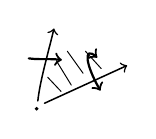
\begin{tikzpicture}[x=1cm,y=1cm,line cap=round,line join=round]
\fill (0,0) circle[radius=.025];
\draw[->,line width=.55pt] (.015,.10) .. controls (.04,.35) and (.16,.76) .. (.22,1.02);
\draw[->,line width=.55pt] (.10,.07)--(1.15,.55);
\draw[line width=.35pt] (.14,.40)--(.31,.22)
 (.25,.61)--(.44,.30)
 (.39,.73)--(.59,.45)
 (.62,.73)--(.82,.51);
\draw[->,line width=.8pt] (-.10,.64) .. controls (.03,.62) and (.14,.64) .. (.32,.62);
\draw[<->,line width=.8pt] (.77,.65) .. controls (.59,.80) and (.62,.56) .. (.81,.23);
\end{tikzpicture}}
) with the generating relations
\[
(25)\qquad
\left\{\begin{aligned}
\unsure{(\sigma_0')^2}&=\unsure{(\sigma_1')^2}=\unsure{(\sigma_2')^2}
=\unsure{(\sigma_2'\sigma_0')^2}=1\\
\unsure{\bigl(\underbrace{\sigma_1'\sigma_0'}_{\rho_f}\bigr)^3}&=1
\end{aligned}\right.
\]

\margin{we could also write $\unsure{\sigma_\infty'}$ instead of $\unsure{\sigma_2'}$.
We would have done better to denote them \inserted{\unsure{here}} outright $r_0,r_1,r_\infty$ (instead of $\sigma_0,\sigma_1,\sigma_2$).}

The subgroup \inserted{$\Pi_{0,3}'$} of index 2 \deleted{\illegible{1}}\inserted{(oriented \unsure{triangul'} cartographic group)} is generated by
\[
\unsure{\sigma_1'\sigma_0'}=\rho_f\inserted{\unsure{=\ell_\infty'}},\qquad
\unsure{\sigma_2'\sigma_1'}=\rho_s\inserted{\unsure{=\ell_0'}},\qquad
\unsure{\sigma_0'\sigma_2'}=\unsure{\sigma'|\sigma}\inserted{\unsure{=\ell_1'}},
\]
with the generating relations
\[
(26)\qquad
\rho_f\sigma\rho_s\deleted{\unsure{\rho_s}}=1
\qquad
\sigma^2=\rho_f^3=1
\]
This is therefore the quotient of $\Pi_{0,3}$ by $\ell_1^2,\ell_\infty^3$
\[
(\unsure{27|17})\qquad
\left\{\begin{array}{rcl}
\Pi_{0,3}&\longrightarrow&\Pi_{0,3}'\\
\ell_0&\longmapsto&\ell_0'=\rho_s\\
\ell_1&\longmapsto&\ell_1'=\sigma\\
\ell_\infty&\longmapsto&\ell_\infty'=\rho_f
\end{array}\right.
\qquad,
\]
\deleted{\illegible{1}} This homomorphism extends to

\deleted{\unsure{(28)|(27)}}

\margin{89}
